\documentclass[
    xcolor={svgnames,dvipsnames},
    hyperref={colorlinks, citecolor=DeepPink4, linkcolor=DarkRed, urlcolor=DarkBlue}
    ]{beamer}  % for hardcopy add 'trans'

\mode<presentation>
{
  \usetheme{Singapore}
  % or ...
  \setbeamercovered{transparent}
  % or whatever (possibly just delete it)
}



\addtobeamertemplate{navigation symbols}{}{%
    \usebeamerfont{footline}%
    \usebeamercolor[fg]{footline}%
    \hspace{1em}%
    \insertframenumber/\inserttotalframenumber
}



\usepackage{fontspec} 
%\usepackage[xcharter]{newtxmath}
%\setmainfont{XCharter}
\usepackage{unicode-math}
%\setmathfont{XCharter-Math.otf}
\setmonofont{DejaVu Sans Mono}[Scale=MatchLowercase] % provides unicode characters 

\usepackage{tikz}
\usetikzlibrary{matrix, shapes, arrows.meta, positioning, fit, backgrounds, calc}

% \usetikzlibrary{matrix, arrows.meta, positioning, calc, backgrounds}

% for tikz
\usepackage{pgfplots}
\usepgfplotslibrary{fillbetween}
\pgfplotsset{compat=1.16}

\usepackage{varwidth}
\usepackage{minted}
\usemintedstyle{friendly}
\setminted[python]{
  fontsize=\small,
  baselinestretch=1.2,
  bgcolor=codebg,
  linenos=false,
  breaklines=true,
  frame=none
}
\setminted[matlab]{
  fontsize=\small,
  baselinestretch=1.2,
  bgcolor=codebg,
  linenos=false,
  breaklines=true,
  frame=none
}
\setminted[julia]{
  fontsize=\small,
  baselinestretch=1.2,
  bgcolor=codebg,
  linenos=false,
  breaklines=true,
  frame=none
}
%\setminted{mathescape, frame=lines, framesep=3mm}
%\newminted{python}{}
%\newminted{c}{mathescape,frame=lines,framesep=4mm,bgcolor=bg}
%\newminted{java}{mathescape,frame=lines,framesep=4mm,bgcolor=bg}
%\newminted{julia}{mathescape,frame=lines,framesep=4mm,bgcolor=bg}
%\newminted{ipython}{mathescape,frame=lines,framesep=4mm,bgcolor=bg}

\usepackage{graphicx}
\usepackage{amsmath, amssymb, amsthm}
\usepackage{bbm}
\usepackage{mathrsfs}
\usepackage{xcolor}
\usepackage{fancyvrb}


% Quotes at start of chapters / sections
\usepackage{epigraph}  
\renewcommand{\epigraphwidth}{6in}

%% Fonts

%\usepackage[T1]{fontenc}
\usepackage{mathpazo}
%\usepackage{fontspec}
%\defaultfontfeatures{Ligatures=TeX}
%\setsansfont[Scale=MatchLowercase]{DejaVu Sans}
%\setmonofont[Scale=MatchLowercase]{DejaVu Sans Mono}
%\setmathfont{Asana Math}
%\setmainfont{Optima}
%\setmathrm{Optima}
%\setboldmathrm[BoldFont={Optima ExtraBlack}]{Optima Bold}

% Some colors

\definecolor{containerblue}{RGB}{66, 133, 244}
\definecolor{leafgreen}{RGB}{52, 168, 83}
\definecolor{textgray}{RGB}{51, 51, 51}
\definecolor{backgroundgray}{RGB}{248, 249, 250}
\definecolor{codebg}{RGB}{241, 241, 241}
\definecolor{aquamarine}{RGB}{69,139,116}
\definecolor{midnightblue}{RGB}{25,25,112}
\definecolor{darkslategrey}{RGB}{47,79,79}
\definecolor{darkorange4}{RGB}{139,90,0}
\definecolor{dogerblue}{RGB}{24,116,205}
\definecolor{blue2}{RGB}{0,0,238}
\definecolor{bg}{rgb}{0.95,0.95,0.95}
\definecolor{DarkOrange1}{RGB}{255,127,0}
\definecolor{ForestGreen}{RGB}{34,139,34}
\definecolor{DarkRed}{RGB}{139, 0, 0}
\definecolor{DarkBlue}{RGB}{0, 0, 139}
\definecolor{Blue}{RGB}{0, 0, 255}
\definecolor{Brown}{RGB}{165,42,42}


\setlength{\parskip}{1.5ex plus0.5ex minus0.5ex}

%\renewcommand{\baselinestretch}{1.05}
%\setlength{\parskip}{1.5ex plus0.5ex minus0.5ex}
%\setlength{\parindent}{0pt}

% Typesetting code
\definecolor{bg}{rgb}{0.95,0.95,0.95}
\newcommand{\Fact}{\textcolor{Brown}{\bf Fact. }}
\newcommand{\Facts}{\textcolor{Brown}{\bf Facts }}
\newcommand{\keya}{\textcolor{turquois4}{\bf Key Idea. }}
\newcommand{\Factnodot}{\textcolor{Brown}{\bf Fact }}
\newcommand{\Eg}{\textcolor{ForestGreen}{Example. }}
\newcommand{\Egs}{\textcolor{ForestGreen}{Examples. }}
\newcommand{\Ex}{{\bf Ex. }}



\renewcommand{\theFancyVerbLine}{\sffamily
    \textcolor[rgb]{0.5,0.5,1.0}{\scriptsize {\arabic{FancyVerbLine}}}}

\newcommand{\navy}[1]{\textcolor{DarkBlue}{\bf #1}}
\newcommand{\brown}[1]{\textcolor{Brown}{\sf #1}}
\newcommand{\green}[1]{\textcolor{ForestGreen}{\sf #1}}
\newcommand{\blue}[1]{\textcolor{Blue}{\sf #1}}
\newcommand{\emp}[1]{\textcolor{DarkOrange1}{\bf #1}}
\newcommand{\red}[1]{\textcolor{Red}{\bf #1}}

% Symbols, redefines, etc.

\newcommand{\code}[1]{\texttt{#1}}

\newcommand{\argmax}{\operatornamewithlimits{argmax}}
\newcommand{\argmin}{\operatornamewithlimits{argmin}}

\DeclareMathOperator{\cl}{cl}
\DeclareMathOperator{\interior}{int}
\DeclareMathOperator{\Prob}{Prob}
\DeclareMathOperator{\determinant}{det}
\DeclareMathOperator{\trace}{trace}
\DeclareMathOperator{\Span}{span}
\DeclareMathOperator{\rank}{rank}
\DeclareMathOperator{\cov}{cov}
\DeclareMathOperator{\corr}{corr}
\DeclareMathOperator{\var}{var}
\DeclareMathOperator{\mse}{mse}
\DeclareMathOperator{\se}{se}
\DeclareMathOperator{\row}{row}
\DeclareMathOperator{\col}{col}
\DeclareMathOperator{\range}{rng}
\DeclareMathOperator{\dimension}{dim}
\DeclareMathOperator{\bias}{bias}


% mics short cuts and symbols
\newcommand{\st}{\ensuremath{\ \mathrm{s.t.}\ }}
\newcommand{\setntn}[2]{ \{ #1 : #2 \} }
\newcommand{\cf}[1]{ \lstinline|#1| }
\newcommand{\fore}{\therefore \quad}
\newcommand{\tod}{\stackrel { d } {\to} }
\newcommand{\toprob}{\stackrel { p } {\to} }
\newcommand{\toms}{\stackrel { ms } {\to} }
\newcommand{\eqdist}{\stackrel {\textrm{ \scriptsize{d} }} {=} }
\newcommand{\iidsim}{\stackrel {\textrm{ {\sc iid }}} {\sim} }
\newcommand{\1}{\mathbbm 1}
\newcommand{\dee}{\,{\rm d}}
\newcommand{\given}{\, | \,}
\newcommand{\la}{\langle}
\newcommand{\ra}{\rangle}

\newcommand{\boldA}{\mathbf A}
\newcommand{\boldB}{\mathbf B}
\newcommand{\boldC}{\mathbf C}
\newcommand{\boldD}{\mathbf D}
\newcommand{\boldM}{\mathbf M}
\newcommand{\boldP}{\mathbf P}
\newcommand{\boldQ}{\mathbf Q}
\newcommand{\boldI}{\mathbf I}
\newcommand{\boldX}{\mathbf X}
\newcommand{\boldY}{\mathbf Y}
\newcommand{\boldZ}{\mathbf Z}

\newcommand{\bSigmaX}{ {\boldsymbol \Sigma_{\hboldbeta}} }
\newcommand{\hbSigmaX}{ \mathbf{\hat \Sigma_{\hboldbeta}} }

\newcommand{\RR}{\mathbbm R}
\newcommand{\NN}{\mathbbm N}
\newcommand{\PP}{\mathbbm P}
\newcommand{\EE}{\mathbbm E \,}
\newcommand{\XX}{\mathbbm X}
\newcommand{\ZZ}{\mathbbm Z}
\newcommand{\QQ}{\mathbbm Q}

\newcommand{\fF}{\mathcal F}
\newcommand{\dD}{\mathcal D}
\newcommand{\lL}{\mathcal L}
\newcommand{\gG}{\mathcal G}
\newcommand{\hH}{\mathcal H}
\newcommand{\nN}{\mathcal N}
\newcommand{\pP}{\mathcal P}





\title{Computational Economics and the AI Revolution}



\author{John Stachurski}


\date{2025}


\begin{document}

\begin{frame}
  \titlepage
\end{frame}



\begin{frame}{Topics}

    \begin{itemize}
        \item Introduction
        \vspace{0.5em}
        \item ANNs and deep learning
        \vspace{0.5em}
        \item Stochastic approximation
        \vspace{0.5em}
        \item Dynamic programming
        \vspace{0.5em}
        \item Reinforcement learning
        \vspace{0.5em}
        \item Economic applications
    \end{itemize}

\end{frame}



\begin{frame}{An AI revolution}

    AI is changing the world

    \begin{itemize}
        \item generative AI  (LLMs, image / music / video generators)
        \vspace{0.5em}
        \item image processing / computer vision
        \vspace{0.5em}
        \item speech recognition, translation
        \vspace{0.5em}
        \item scientific knowledge discovery
        \vspace{0.5em}
        \item forecasting and prediction 
        \vspace{0.5em}
        \item etc
    \end{itemize}

    
\end{frame}


\begin{frame}
    
    \begin{figure}
       \centering
       \scalebox{0.24}{
\includegraphics[trim={0cm 0cm 0cm 0cm},clip]{alpha_fold.pdf}}
    \end{figure}

\end{frame}

\begin{frame}\frametitle{AlphaFold}

    \begin{itemize}
        \item AI system by DeepMind that predicts protein structures
            \vspace{0.5em}
        \item Open-sourced code and database for global access
            \vspace{0.5em}
        \item Accelerating drug discovery and design
            \vspace{0.5em}
        \item Enabling research on diseases like cancer and Alzheimer's
            \vspace{0.5em}
        \item Supporting enzyme engineering for sustainability
    \end{itemize}

            \vspace{0.5em}
            \vspace{0.5em}
            \vspace{0.5em}
    2024 Nobel Prize in Chemistry awarded to Demis Hassabis and John
    Jumper for development of AlphaFold

\end{frame}

\begin{frame}
    \frametitle{LLMs}
    
    \begin{figure}
       \centering
       \scalebox{0.24}{
\includegraphics[trim={0cm 0cm 0cm 0cm},clip]{llms.png}}
    \end{figure}

\end{frame}


\begin{frame}
    \frametitle{Image Generators}
    
    \begin{figure}
       \centering
       \scalebox{0.3}{
\includegraphics[trim={0cm 0cm 0cm 0cm},clip]{image_gen.pdf}}
    \end{figure}

\end{frame}


\begin{frame}
    \frametitle{Weather forecasts}
    
    \begin{figure}
       \centering
       \scalebox{0.22}{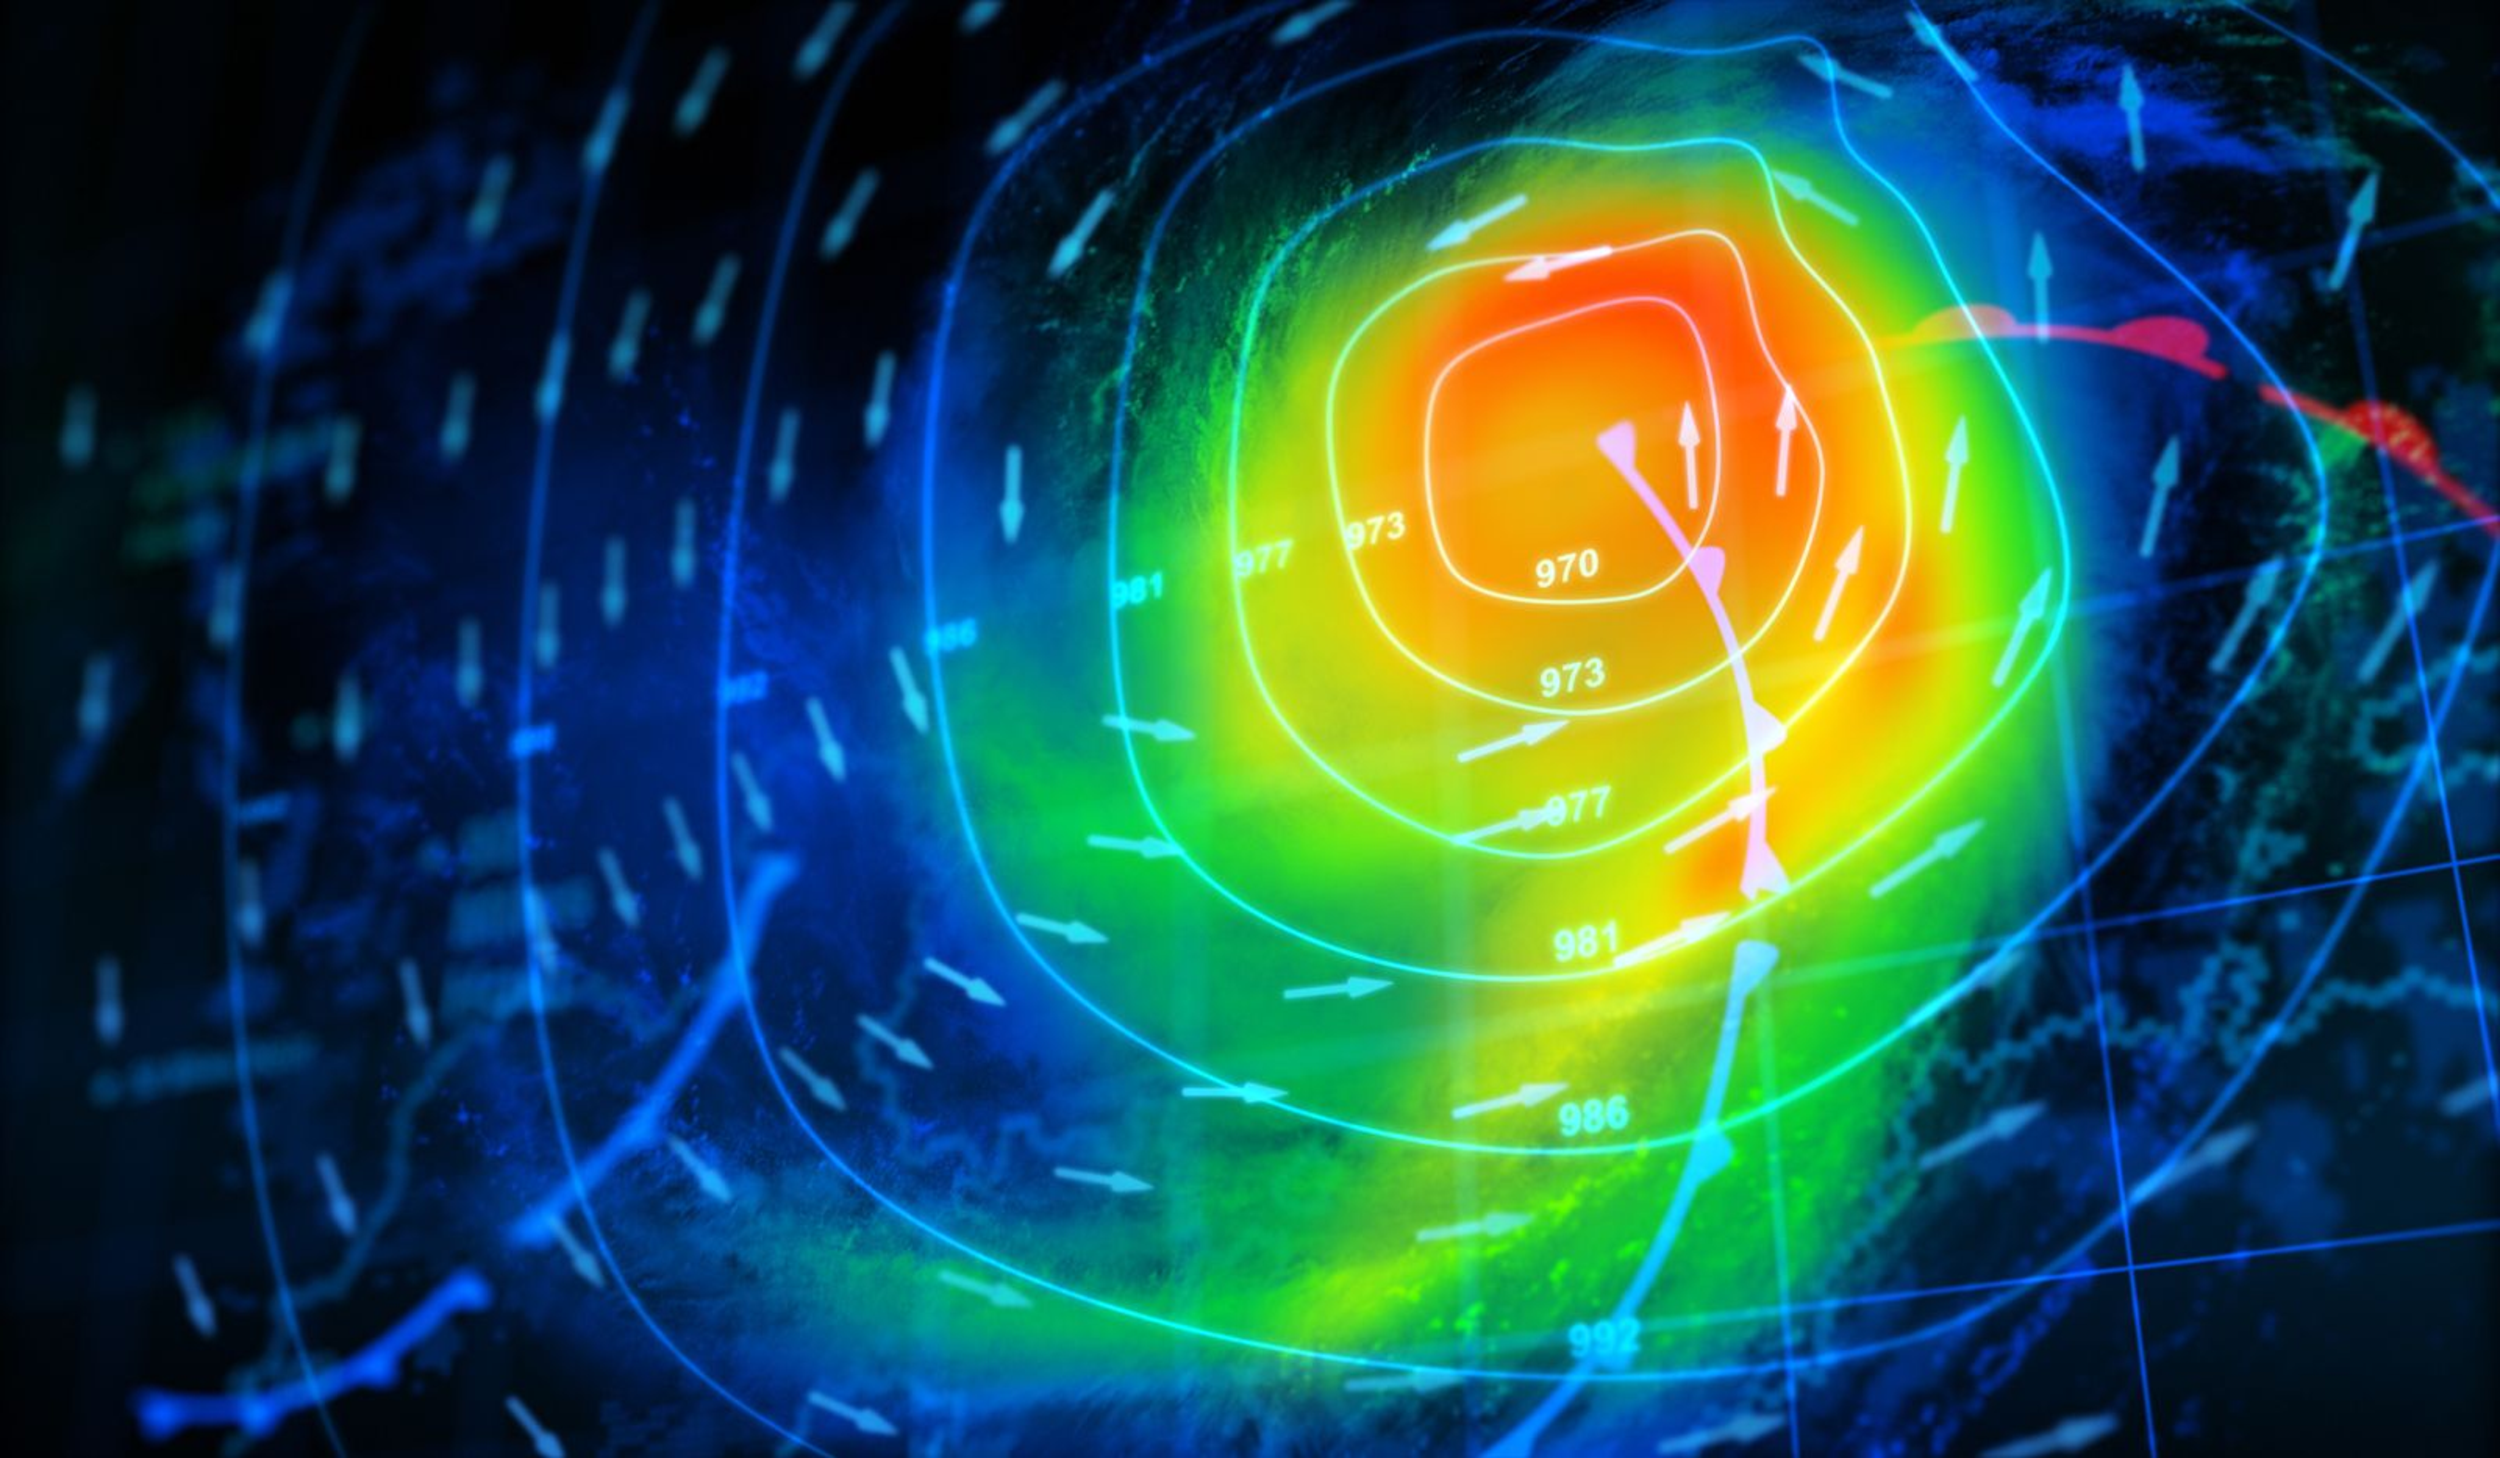
\includegraphics[trim={0cm 0cm 0cm 0cm},clip]{weather.pdf}}
    \end{figure}

\end{frame}


\begin{frame}

    
    ``ECMWF's weather forecasting model is considered the gold standard for
        medium-term weather forecasting\ldots 
        Google DeepMind claims to beat it 90\% of the time\ldots''

    \vspace{0.5em}
    \vspace{0.5em}

    ``Traditional forecasting models are big, complex computer algorithms based
    on atmospheric physics and take hours to run. AI models can create forecasts
    in just seconds.'' 
    \vspace{0.5em}
    \vspace{0.5em}

    $\quad \qquad$$\quad \qquad$ Source: MIT Technology Review  July 2024



\end{frame}



\begin{frame}
    \frametitle{Translation Engines}
    
    \begin{figure}
       \centering
       \scalebox{0.42}{
\includegraphics[trim={0cm 0cm 0cm 0cm},clip]{translation.pdf}}
    \end{figure}

\end{frame}


\begin{frame}{Killer drones, Skynet, etc.}

    \begin{figure}
       \centering
       \scalebox{0.46}{
\includegraphics[trim={0cm 0cm 0cm 0cm},clip]{terminator.png}}
    \end{figure}

\end{frame}

\begin{frame}{Investment}

    Private AI investment in 2024:

    \begin{itemize}
        \item U.S. = \$109 billion 
        \vspace{0.5em}
        \item China \$9.3 billion 
        \vspace{0.5em}
        \item UK \$4.5 billion
    \end{itemize}

        \vspace{0.5em}
        \vspace{0.5em}
    Massive investments in 

    \begin{itemize}
        \item data centers
        \vspace{0.5em}
        \item GPU design and production
        \vspace{0.5em}
        \item software development
    \end{itemize}

\end{frame}


\begin{frame}
    
    What kinds of problems are they trying to solve?

\end{frame}




\begin{frame}
    \frametitle{Deep learning in two slides}
    
    Aim: approximate an unknown functional relationship
    %
    \begin{equation*}
        y = f(x)
        \qquad (x \in \RR^k, \; y \in \RR)
    \end{equation*}

    \Egs
    %
    \begin{itemize}
        \item $x = $ cross section of returns today, $y = $ return on oil futures tomorrow
        \vspace{0.5em}
        \item $x = $ weather sensor data today, $y = $ max temp tomorrow
    \end{itemize}
        \vspace{0.5em}
        \vspace{0.5em}

    Problem:

    \begin{itemize}
        \item observe $(x_i, y_i)_{i=1}^n$ and seek $f$ such that $y_{n+1}
            \approx f(x_{n+1})$
    \end{itemize}

\end{frame}


\begin{frame}

    Deep learning is nonlinear regression: 

    \begin{enumerate}
        \item Choose function class $\{f_\theta\}_{\theta \in \Theta}$ 
            \vspace{0.4em}
        \item Minimize loss over the parameter space, where
            %
            \begin{equation*}
                \ell(\theta) := \sum_{i=1}^n (y_i - f_\theta(x_i))^2
                \quad \st \quad \theta \in \Theta
            \end{equation*}
    \end{enumerate}


    \pause
    \vspace{0.5em}
    In the case of ANNs, elements of $\{f_\theta\}_{\theta \in \Theta}$
    have a particular structure

    \begin{itemize}
        \item we discuss this structure soon
        \vspace{0.5em}
        \item typically, $\theta \mapsto f_\theta(x)$ is smooth for all $x$
        \vspace{0.5em}
        \item MSE is a popular loss function but others are also used
    \end{itemize}

\end{frame}


\begin{frame}
    

    Minimizing a smooth loss functions  -- what algorithm?
    
    \begin{figure}
       \begin{center}
        \scalebox{0.15}{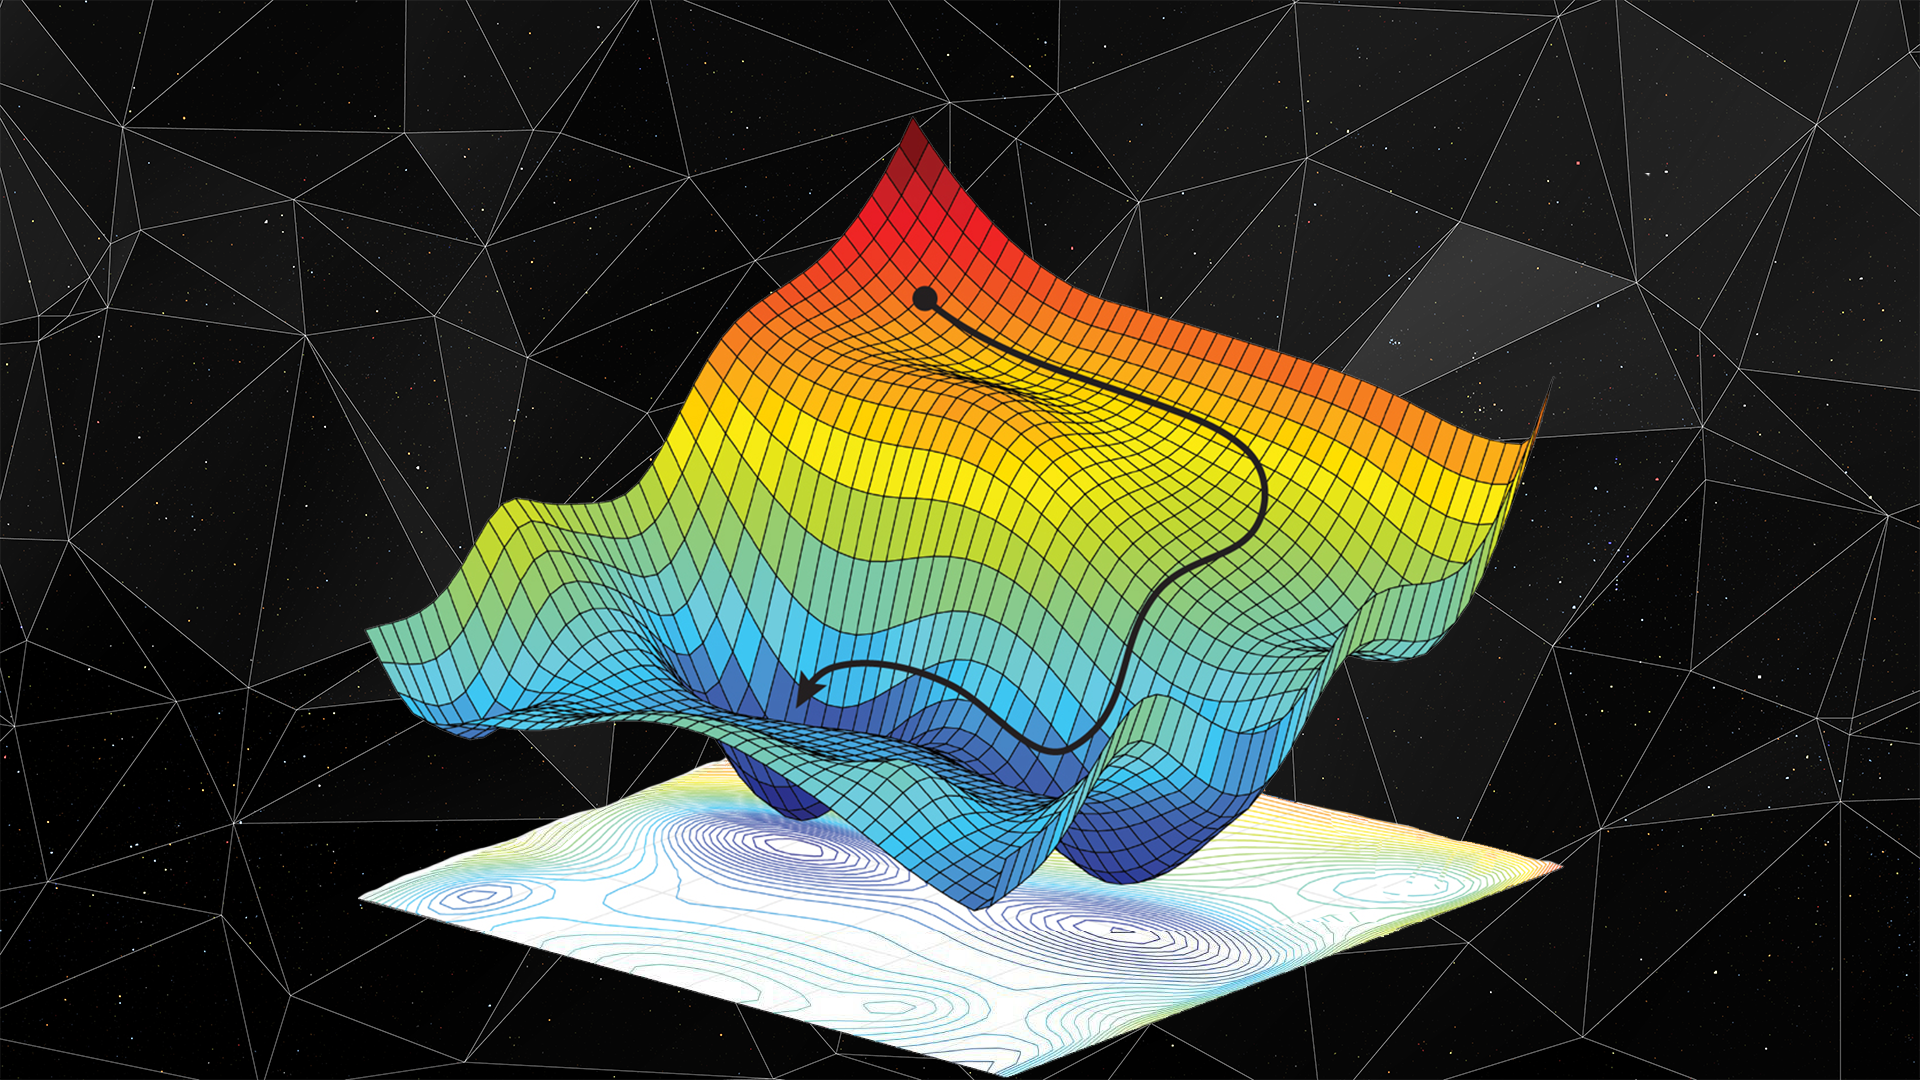
\includegraphics[trim={0cm 0cm 0cm 0cm},clip]{gdi.png}}
       \end{center}
    \end{figure}

    Source: \url{https://danielkhv.com/}

\end{frame}


\begin{frame}

    Deep learning: $\theta \in \RR^d$ where $d = ?$
    
    \begin{figure}
       \begin{center}
        \scalebox{0.14}{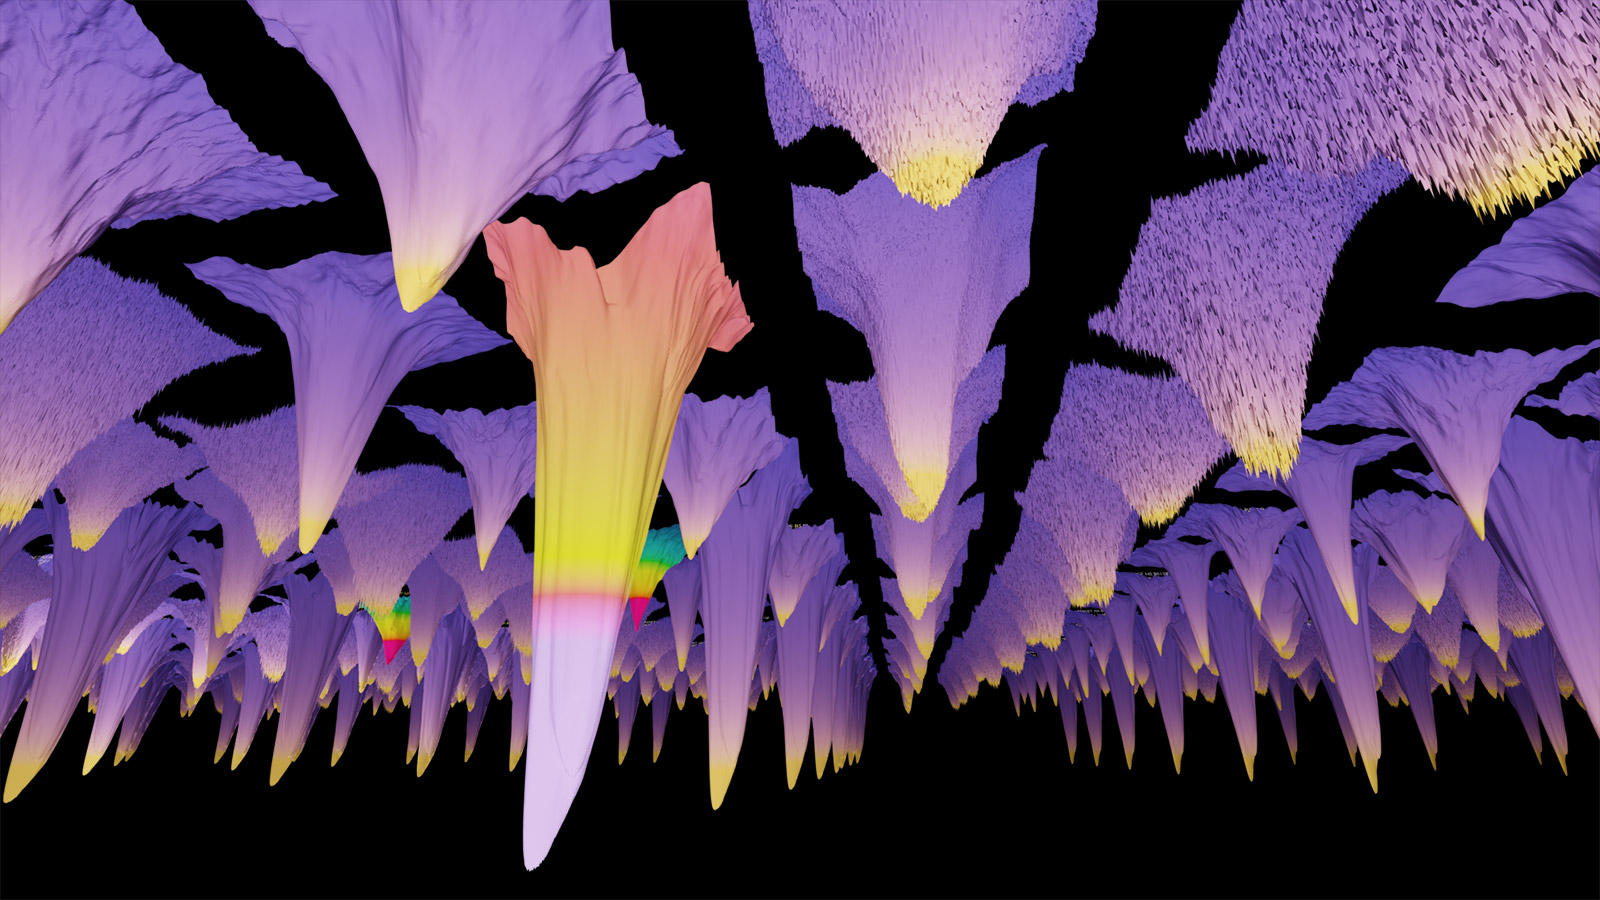
\includegraphics[trim={0cm 0cm 0cm 0cm},clip]{loss2.jpg}}
       \end{center}
    \end{figure}

    Source: \url{https://losslandscape.com/gallery/}

\end{frame}




\begin{frame}
    \frametitle{How does it work?}
    
    How is it possible to minimize loss over such high dimensions??

        \vspace{0.5em}
        \vspace{0.5em}
        \vspace{0.5em}
        \vspace{0.5em}
        \pause

    Core elements
    %
    \begin{itemize}
        \item automatic differentiation (for \underline{gradient} descent)
        \vspace{0.5em}
        \item parallelization (GPUs or TPUs)
        \vspace{0.5em}
        \item Compilers / JIT-compilers
    \end{itemize}

\end{frame}

\begin{frame}[fragile]
    \frametitle{Automatic differentiation}

    \vspace{0.5em}
    ``Exact numerical'' differentiation
    
    \begin{minted}{python}

def loss(θ, x, y):
  return jnp.sum((y - f(θ, x))**2)

loss_gradient = grad(loss)
dθ = loss_gradient(θ, x_data, y_data)
θ = θ - λ * dθ

    \end{minted}



\end{frame}


\begin{frame}[fragile]
    \frametitle{Parallelization}

    \begin{figure}
       \begin{center}
        \scalebox{0.18}{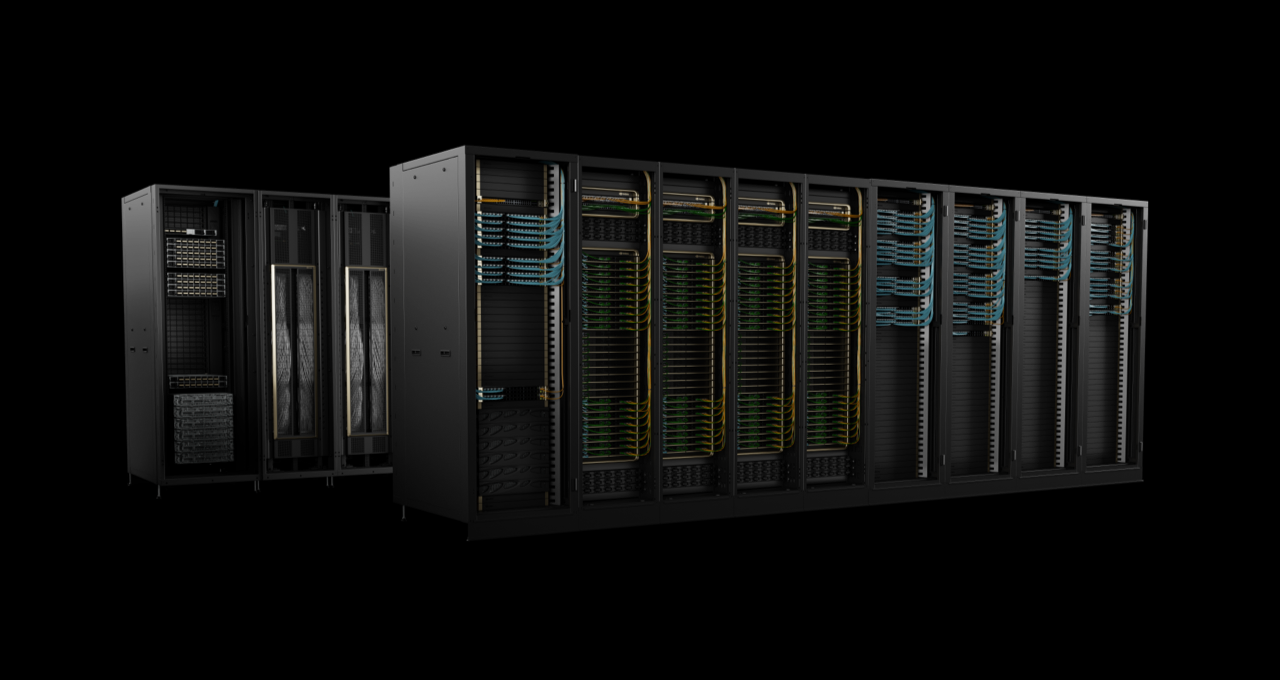
\includegraphics[trim={0cm 0cm 0cm 0cm},clip]{dgx.png}}
       \end{center}
    \end{figure}
    
\end{frame}


\begin{frame}[fragile]

    Multithreading and multiprocessing


    \vspace{0.5em}
    \begin{itemize}
        \item multithreading over GPU cores (how many?)
    \end{itemize}
    
    \begin{minted}{python}
vectorized_function = vmap(function)  
outputs = vectorized_function(data)  
    \end{minted}

    \vspace{0.5em}
    \vspace{0.5em}
    \begin{itemize}
        \item multiprocessing over accelerators in a GPU farm / cluster 
    \end{itemize}

    \begin{minted}{python}
parallel_function = pmap(function)  
outputs = parallel_function(data)  
    \end{minted}



\end{frame}


\begin{frame}[fragile]
    \frametitle{Just-in-time compilers}

    \vspace{0.5em}
    
    \begin{minted}{python}
@jit
def f(x):
    return jnp.sin(x) - jnp.cos(x**2)
    \end{minted}

    \vspace{0.5em}
    Advantages over AOT compilers:

    \begin{itemize}
        \item cleaner code
    \vspace{0.5em}
        \item more portable
    \vspace{0.5em}
        \item automatic parallelization (same code for CPUs / GPUs)
    \end{itemize}

\end{frame}



\begin{frame}
    \frametitle{Platforms}
    
    Platforms that support AI / deep learning:

    \vspace{0.5em}
    \begin{itemize}
        \item Tensorflow
        \vspace{0.5em}
        \item \brown{PyTorch} (Llama, ChatGPT)
        \vspace{0.5em}
        \item \brown{Google JAX} (Gemini, DeepMind)
        \vspace{0.5em}
        \item Keras (backends $=$ JAX, PyTorch)
        \vspace{0.5em}
        \item Mojo? (Modular (Python))
        \vspace{0.5em}
        \item MATLAB? 
    \end{itemize}

\end{frame}




\begin{frame}
    
    Popularity -- languages
    
    \begin{figure}
       \begin{center}
        \scalebox{0.62}{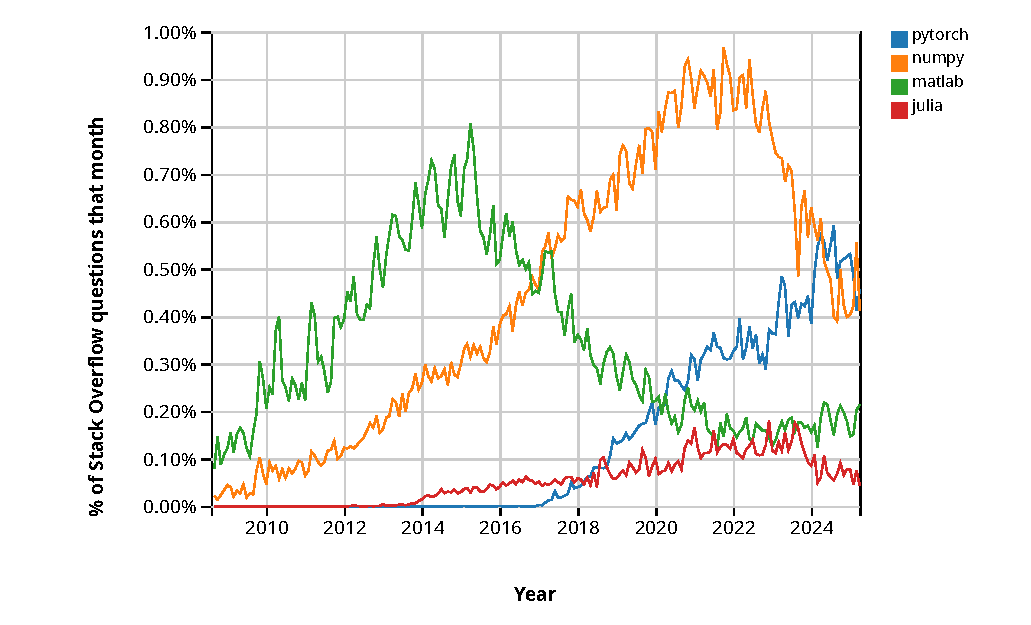
\includegraphics[trim={0cm 0cm 0cm 0cm},clip]{trends.pdf}}
       \end{center}
    \end{figure}

\end{frame}


\begin{frame}
    
    Popularity -- deep learning frameworks
    
    \begin{figure}
       \begin{center}
        \scalebox{0.62}{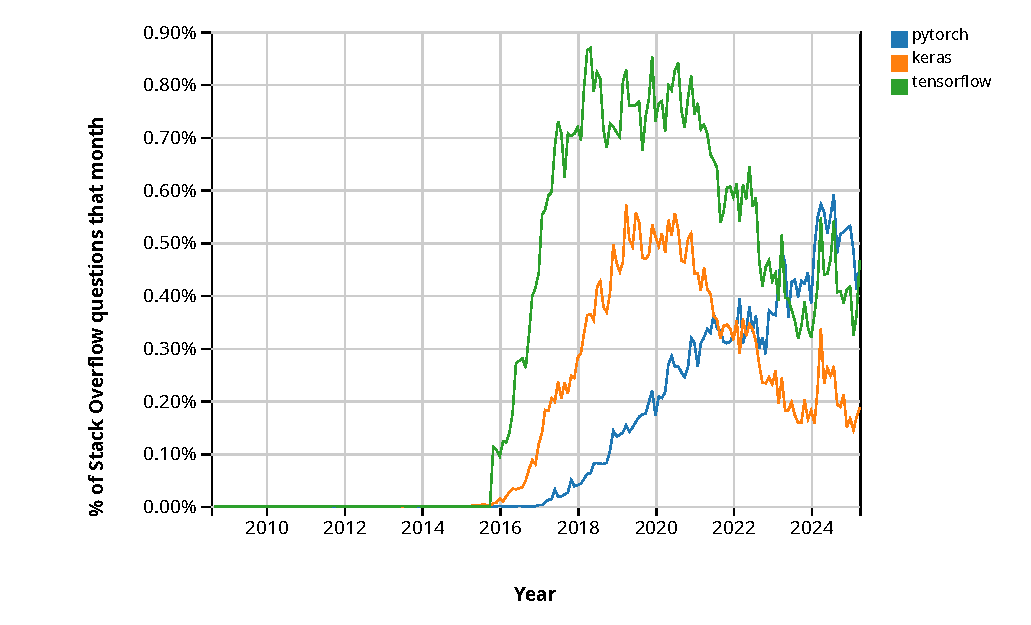
\includegraphics[trim={0cm 0cm 0cm 0cm},clip]{trends_2.pdf}}
       \end{center}
    \end{figure}

\end{frame}



\begin{frame}{AI for coding}
    
    \begin{figure}
       \centering
       \scalebox{0.36}{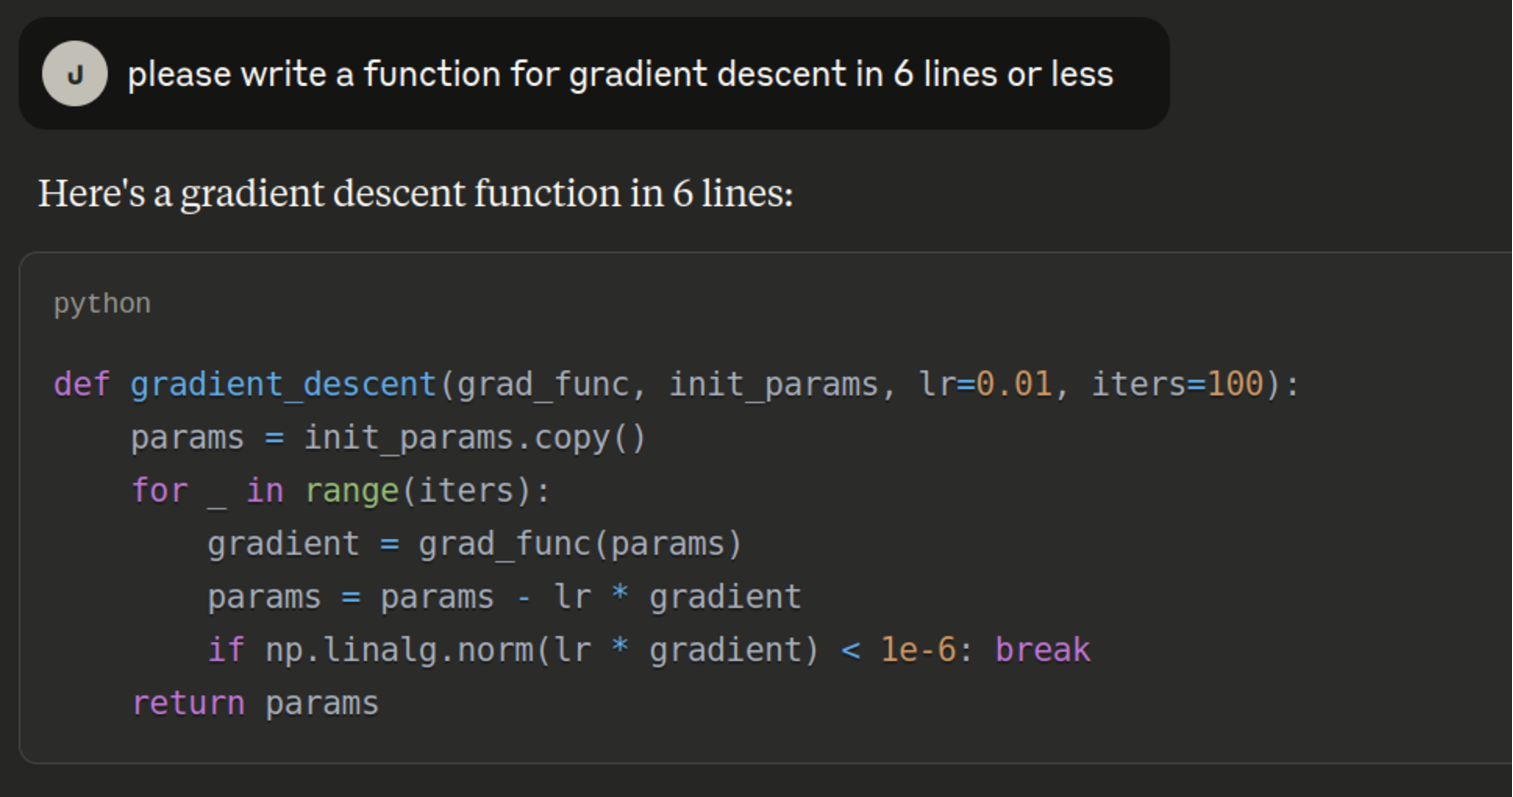
\includegraphics[trim={0cm 0cm 0cm 0cm},clip]{code_ai.pdf}}
    \end{figure}

\end{frame}


\begin{frame}{Affects language choice}
    
    ``I'm definitely stronger with Python than MATLAB.''

    \vspace{0.5em}
    ``My capabilities with Python
    are more comprehensive. I have deeper familiarity with Python's extensive
    ecosystem of libraries, frameworks, and modern development practices.''


    \vspace{0.5em}
    ``I can
    more confidently help with advanced Python topics, debugging complex Python
    code, and implementing Python best practices.''

\end{frame}

\begin{frame}
    
    ``I'm definitely stronger with Python than Julia.''

    \vspace{0.5em}
    ``Python is one of my most proficient languages - I have deep familiarity with
    its syntax, libraries, frameworks, and best practices across many domains
    including data science, web development, machine learning, and
    general-purpose programming.''

    \vspace{0.5em}
    ``While I understand Julia's syntax and core concepts, my expertise with it
    isn't as comprehensive as with Python.''

\end{frame}

\begin{frame}

    Thoughts from developer \texttt{Lonely-Public2655}

    \begin{itemize}
        \item AI doesn't see the big picture 
        \vspace{0.5em}
        \item Can ace small tasks but struggles to connect them meaningfully
        \vspace{0.5em}
        \item You still need to be the architect
        \vspace{0.5em}
        \item Context is fragile: AI forgets. A lot.
        \vspace{0.5em}
        \item Once things get weird, AI starts guessing
        \vspace{0.5em}
        \item Sometimes AI gets really weird 
    \end{itemize}

\end{frame}


\begin{frame}
    \frametitle{AI tools for economic modeling}

    Let's say that you want to do computational economics without deep learning

    \vspace{0.5em}
    Can these new AI tools be applied?

    \pause

    \vspace{0.5em}
    \vspace{0.5em}
    \emp{Yes!}
    \emp{Yes!}
    \emp{Yes!}

    \begin{itemize}
        \item fast matrix algebra
        \vspace{0.5em}
        \item fast solutions to linear systems
        \vspace{0.5em}
        \item fast nonlinear system solvers
        \vspace{0.5em}
        \item fast optimization, etc.
    \end{itemize}


\end{frame}



\begin{frame}
    \frametitle{Case Study}

    The CBC uses the ``overborrowing'' model of Bianchi (2011)

    \begin{itemize}
        \item credit constraint loosens during booms
        \item bad shocks $\to$ sudden stops
    \end{itemize}

    \vspace{0.5em}
    CBC implementation in MATLAB 

    \begin{itemize}
        \item runs on \$10,000 mainframe with 356 CPUs and 1TB RAM
        \item runtime $=$ 12 hours
    \end{itemize}

    \pause
    \vspace{0.5em}
    Rewrite in Python + Google JAX

    \begin{itemize}
        \item runs on \$400 gaming GPU with 10GB RAM
        \item runtime $=$ 7 seconds
    \end{itemize}


\end{frame}



\end{document}


